\chapter{ECG: Electrocardiogram}
In this experience we built an electrocardiograph and tested it on a group member.

\section{Materials}
\begin{itemize}
\item Operational amplifiers OP07
\item Instrumentation amplifier (INA) AD622
\item Resistors, trimmers
\item Power supply RIGOL DP831A
\item Waveform generator RIGOL DG1032
\item Multimeter RIGOL DM3068
\item Isolation amplifier ISO124
\item Three electrodes
\item $9$ V Batteries
\end{itemize}
All resistors and capacitors used had  an uncertainty of 5\% of their value.

\section{Experimental setup}
All the circuit connected with the patient was powered using a 9 V battery: thinking of a real situation in fact, we prevent this way the patient to be exposed to the electrical grid voltage of 220 V in case of any instrumentation malfunctioning.\\
The signal we wanted to acquire from the electrodes had a frequency of nearly 1.25 Hz and an amplitude from 1 to 4 mV, with an offset of 0.7/0.8 V due to the internal electrodes potential. Obviously any cable or body movement would interfere with the measurement, generating some kind of current, and it is also important to keep in mind the presence of parasite capacitance and inductance. For these reasons our circuit needs to remove the common potential and reduce as much noise as possible, without removing signals at 1.25 Hz frequencies.\\
\begin{figure}[H]
\centering
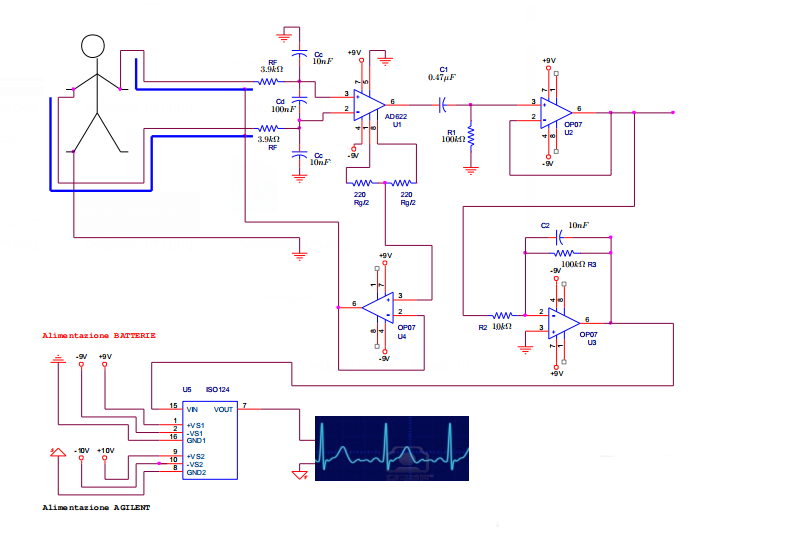
\includegraphics[width=.8\textwidth]{8/circuit.png}
\caption{Circuit designed}
\end{figure}
The  first step was to remove high frequency noise by using two low-pass filters before the OP07 inputs: this was achieved by the use of two $3.9 k\Omega$ resitors ($R_F$) and three capacitors as shown in figure 7.1 (one connecting the two resistors of 100 nF ($C_D$), the others of 10 nF ($C_C$)).\\
Then we removed the common signal thanks to a differential amplifier, we set the component's gain to $G =   \frac{50.1 k\Omega}{R_G} + 1 = 116$, where $R_G = 440 \Omega$ is the total resistance between pin 1 and 8. This resistance was obtained with two identical resistors in series: this way the voltage between them would have come to be equal to the cable one, so we brought this potential to the coaxial cable shield using a follower for the impedence mismatching. We did this in order to limit the electric dispersion of our signal: if a cable and its shield share the same potential, there will be less electrons that flows from one to the other and so the signal travelling will be better preserved.\\
After that we put the signal through a high-pass filter in order to remove other components and then we used a follower for the impedance mismatching. The next step was a second low-pass filter, but active now. At this time we had the signal we needed, except that we wanted to see it with the oscilloscope, powered with undesired 220 V: in order to separate this "dangerous" component from the rest of the circuit we used the isolation amplifier ISO124.
We took a last precaution: since also skin has a resistance that lowers the signal, we cleaned with alcohol the surface where we attached the electrodes, in the prospective of removing the fat and reducing this resistance.
Like every other object that produces a ddp, a reference ground voltage was needed for the patient: besides the two electrodes on the wrists, we used also a third one on the left ankle to be used as common reference.

\section{Data analysis}
In the circuit there were many filters for reducing noises, but even with all those precautions we still had some noise at nearly 150 Hz, so we decided to smooth the signal with a running mean algorithm. The result is shown in figure 7.2
\begin{figure}[H]
\centering
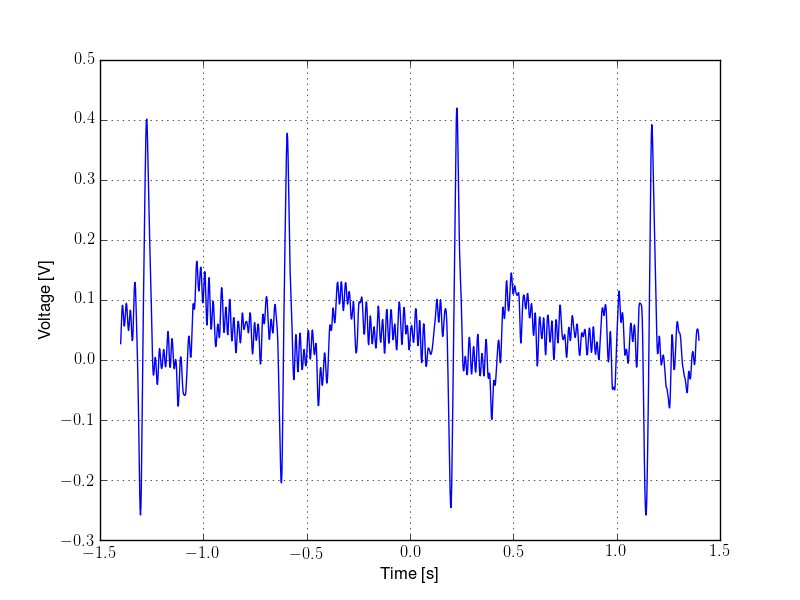
\includegraphics[width=.7\textwidth]{8/ecg.png}
\caption{Signal measured smoothed}
\end{figure}
